\documentclass[letterpaper,11pt]{article}

\usepackage[utf8]{inputenc}
\usepackage[UKenglish]{isodate}
\usepackage{graphicx}
\usepackage{scalerel}
\usepackage{fontawesome5}
\usepackage{lmodern,textcomp}
\usepackage[greek,english]{babel}
\usepackage{alphabeta}
\usepackage{latexsym}
\usepackage[empty]{fullpage}
\usepackage{titlesec}
\usepackage{marvosym}
\usepackage{soul}
\usepackage[dvipsnames]{xcolor}
\usepackage{verbatim}
\usepackage{enumitem}
\usepackage{xcolor}
\usepackage[hidelinks]{hyperref}
\hypersetup{
colorlinks=true,
linkcolor=magenta,
filecolor=magenta,      
urlcolor=cyan,
pdftitle={[Christos Karaneen]CV},
pdfpagemode=FullScreen,
}
\usepackage{fancyhdr}
\usepackage[english]{babel}
\usepackage{tabularx}
\usepackage{pdfcomment}

\pagestyle{fancy}
\fancyhf{} % clear all header and footer fields
\fancyfoot{}
\setlength{\footskip}{4.08003pt}
\renewcommand{\headrulewidth}{0pt}
\renewcommand{\footrulewidth}{0pt}

% Adjust margins
\addtolength{\oddsidemargin}{-0.5in}
\addtolength{\evensidemargin}{-0.5in}
\addtolength{\textwidth}{1in}
\addtolength{\topmargin}{-.5in}
\addtolength{\textheight}{1.0in}

\urlstyle{same}

\raggedbottom
\raggedright
\setlength{\tabcolsep}{0in}

% Sections formatting
\titleformat{\section}{
  \vspace{-4pt}\scshape\raggedright\large
}{}{0em}{}[\color{black}\titlerule \vspace{-5pt}]

%-------------------------
% Custom commands

\newcommand\blfootnote[1]{%
  \begingroup
  \renewcommand\thefootnote{}\footnote{#1}%
  \addtocounter{footnote}{-1}%
  \endgroup
}

\newcommand{\resumeItem}[2]{
  \item\small{
    \textbf{#1}{: #2 \vspace{-2pt}}
  }
}

\newcommand{\resumeSubheading}[4]{
  \vspace{-1pt}\item
    \begin{tabular*}{0.97\textwidth}[t]{l@{\extracolsep{\fill}}r}
      \textbf{#1} & #2 \\
      \textit{\small#3} & \textit{\small #4} \\
    \end{tabular*}\vspace{-5pt}
}

\newcommand{\resumeSubSubheading}[2]{
    \begin{tabular*}{0.97\textwidth}{l@{\extracolsep{\fill}}r}
      \textit{\small#1} & \textit{\small #2} \\
    \end{tabular*}\vspace{-5pt}
}

\newcommand{\resumeSubItem}[2]{\resumeItem{#1}{#2}\vspace{-4pt}}

\renewcommand{\labelitemii}{$\circ$}

\newcommand{\resumeSubHeadingListStart}{\begin{itemize}[leftmargin=*]}
\newcommand{\resumeSubHeadingListEnd}{\end{itemize}}
\newcommand{\resumeItemListStart}{\begin{itemize}}
\newcommand{\resumeItemListEnd}{\end{itemize}\vspace{-5pt}}

%-------------------------------------------
%%%%%%  CV STARTS HERE  %%%%%%%%%%%%%%%%%%%%%%%%%%%%


\begin{document}

%----------HEADING-----------------
\begin{tabular*}{\textwidth}{l@{\extracolsep{\fill}}r}
  \textbf{\Large \href{https://raw.githubusercontent.com/ckaraneen/cv/master/cv.pdf}{\color{black}{Christos Karaneen}}} (Karageorgiou Kaneen) \\
  \textit{\color{black}{Neuroscience \& AI Researcher, Software Engineer}} &
  \href{mailto:ckaraneen@gmail.com}{\raisebox{-0.1em}{\textcolor{YellowOrange}{\small{\faIcon{envelope}}}} ckaraneen@gmail.com}\\
  \href{https://www.github.com/ckaraneen}{{\textcolor{black}{\small{\faIcon{github}}}} github.com/ckaraneen} & \small{(\textit{email me for} \textcolor{Green}{\small{\faIcon{phone}}})} \\
  \href{https://www.linkedin.com/in/ckaraneen/}{linked\raisebox{-0.05em}{\textcolor{RoyalBlue}{\small{\faIcon{linkedin}}}}.com/in/ckaraneen} \\
  \href{https://x.com/ckaraneen}{\raisebox{-0.1em}{\textcolor{Cyan}{
\includegraphics[height=1em]{icons/x_twitter.png}}}.com/ckaraneen} \\
  
\end{tabular*}


%-----------EDUCATION-----------------
\section{Education}
\resumeSubHeadingListStart
\resumeSubheading
      {\href{https://www.uoc.gr/en/home/}{\raisebox{-0.2em}{
\includegraphics[height=1.2em]{icons/uoc.jpg}} University of Crete}}{\href{https://en.wikipedia.org/wiki/Heraklion}{Heraklion, GR}}
      {\href{https://www.neurosciences.med.uoc.gr/index.php/en}{\color{black}{M.Sc., Neuroscience, School of Medicine}}}{Oct. 2021 - Feb. 2024}
\resumeSubheading
      {\href{https://www.tuc.gr/en/home}{\raisebox{-0.1em}{
\includegraphics[height=1.2em]{icons/tuc.jpg}} Technical University of Crete} \label{TUCMarker}}{\href{https://en.wikipedia.org/wiki/Chania}{Chania, GR}}
      {\href{https://www.ece.tuc.gr/en/home}{\color{black}{M.Eng., School of Electrical \& Computer Engineering}}}{Sept. 2014 - Dec. 2019}
\resumeSubHeadingListEnd

%-----------RESEARCH EXPERIENCE-----------------
\section{Research Experience}
  \resumeSubHeadingListStart
    \resumeSubheading
      {\href{https://www.arkabanerjeelab.com/}{\raisebox{-0.3em}{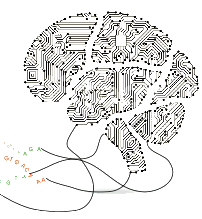
\includegraphics[height=1.5em]{icons/brainwire.png}} Banerjee Lab}, \href{https://www.cshl.edu/}{\raisebox{-0.3em}{
\includegraphics[height=1.5em]{icons/cshl.png}} Cold Spring Harbor Laboratory} \label{BanerjeeLabMarker}}{\href{https://en.wikipedia.org/wiki/Cold_Spring_Harbor,_New_York}{New York, USA}}
      {Neuroscience \& AI Researcher (\hyperref[CSHLNeuroAIResearchInternFundingMarker]{NeuroAI Research Intern})}{June 2024 - Nov. 2024}
      \newline Explored how learned behavior evolves into instinct. See \hyperref[BrainNeuroAIWorkshop2024PosterMarker]{poster}.
    \resumeSubheading
      {\href{http://kordinglab.com/}{\raisebox{-0.2em}{
\includegraphics[height=1em]{icons/kordinglab.jpg}} Kording Lab}, \href{https://www.upenn.edu/}{\raisebox{-0.2em}{
\includegraphics[height=1.3em]{icons/upenn.jpg}} University of Pennsylvania} \label{KordingLabMarker}}{\href{https://en.wikipedia.org/wiki/Philadelphia}{Philadelphia, USA}}
      {Neuroscience \& AI Researcher (\hyperref[UPennVisitingScholarFundingMarker]{Visiting Scholar})}{Dec. 2022 - March 2023}
      \newline Investigated how meta-learning synaptic plasticity rules can best approximate gradient descent. \newline See \hyperref[MLSS2024PosterMarker]{poster} and \hyperref[NeuroscienceMScThesisMarker]{thesis}.
    \resumeSubheading
      {\href{https://dendrites.gr/}{\raisebox{-0.2em}{
\includegraphics[height=1em]{icons/poirazilab.jpg}} Poirazi Lab}, \href{https://www.imbb.forth.gr/en/}{\raisebox{-0.2em}{
\includegraphics[height=1em]{icons/imbb.jpg}} IMBB-FoRTH} \label{PoiraziLabMarker}}{\href{https://en.wikipedia.org/wiki/Heraklion}{Heraklion, GR}}
      {Neuroscience \& AI Researcher (Intern, \hyperref[IMBBFoRTHFellowshipMarker]{M.Sc. Fellow})}{July 2022 - April 2024}
      \begin{itemize}
        \setlength\itemsep{-0.3em}
        \item Examined the computational properties of dendrites. See \href{https://github.com/ckaraneen/nobrianer/blob/main/nobrianer.ipynb}{nobrianer}.
        \item Continued the work I started at the \hyperref[KordingLabMarker]{Kording Lab}. See \hyperref[MLSS2024PosterMarker]{poster} and \hyperref[NeuroscienceMScThesisMarker]{thesis}.
      \end{itemize}
    \resumeSubHeadingListEnd
%-----------INDUSTRY WORK EXPERIENCE-----------------
\section{Industry Work Experience}
  \resumeSubHeadingListStart
    \resumeSubheading
      {\href{https://mist.io/}{\raisebox{-0.2em}{
\includegraphics[height=1em]{icons/mistio.jpg}} mist.io} \normalfont \small{(}\small{\href{https://www.ekathimerini.com/economy/1222675/us-firms-buying-greek-startups/}{\textcolor{gray}{acquired by }}\href{https://www.dell.com/}{\textcolor{cyan}{\raisebox{-0.2em}{
\includegraphics[height=1em]{icons/dell.jpg}} Dell}})}}{Remote}
      {Software \& Infrastructure Engineer}{April 2021 - July 2022}
      \resumeItemListStart
        \resumeItem{Platform features and issues}
        {Developed features and addressed issues having to do with machines, stacks, networks, scripts and other resources managed by the platform within the \textit{api} and \textit{tests} submodules of both community and enterprise editions. See \href{https://github.com/mistio/mist.api/commits?author=ckarageorgkaneen@gmail.com}{my contributions on mist-ce}.}
        \resumeItem{Third-party company tests}
        {Outlined and implemented the API and functional tests of a distributed micro-services client project for \href{https://www.juniper.net/}{\raisebox{-0.3em}{
\includegraphics[height=1.2em]{icons/juniper.jpg}}}}
      \resumeItemListEnd
    \resumeSubheading
      {\href{https://grnet.gr/en/}{\raisebox{-0.2em}{
\includegraphics[height=1em]{icons/grnet.jpg}} Greek Research \& Technology Network}}{Remote}
      {Software Engineer \& Maintainer}{May 2020 - April 2021}
      \newline Contributed to reducing Greece's public sector bureaucracy: built, alongside one lead developer, and maintained the v1 of \href{https://en.mitos.gov.gr/}{\raisebox{-0.2em}{
\includegraphics[height=1em]{icons/mitos.jpg}} mitos}: the Greek National Registry of Public Services (Εθνικό Μητρώο Διαδικασιών). See \href{https://github.com/ckaraneen/diavlos}{diavlos}.
    \resumeSubheading
      {\href{https://www.myrmex-inc.com/}{\raisebox{-0.2em}{
\includegraphics[height=1em]{icons/myrmex.jpg}} Myrmex} \normalfont \small{(}\small{\href{https://www.ekathimerini.com/economy/1185079/britains-ocado-buys-out-greek-startup-myrmex/}{\textcolor{gray}{acquired by }}\href{https://www.ocado.com}{\textcolor{violet}{\raisebox{-0.2em}{
\includegraphics[height=1em]{icons/ocado.jpg}} Ocado}})}}{\href{https://en.wikipedia.org/wiki/Athens}{Athens, GR}}
      {Software Engineer}{Sept. 2019 - March 2020}
      \resumeItemListStart
        \resumeItem{Power-monitoring application}
        {Created a GUI that displays in real time the battery state of each robot.}
        \resumeItem{gRPC clients}
        {Ported gRPC client proxies for the APIs of two key system components.}
        \resumeItem{Bug-reporting tool}
        {Implemented a bug-reporting tool that automatically gathers diagnostics whenever a bug or issue arises, decreasing the time required to collect data from more than 20 min. down to 15 sec.}
      \resumeItemListEnd
  \resumeSubHeadingListEnd
%-----------ENGINEERING INTERNSHIP Experience-----------------
\section{Engineering Internship Experience}
  \resumeSubHeadingListStart
    \resumeSubheading
      {\href{https://www.projekte.hu-berlin.de/en/larkum}{\raisebox{-0.2em}{
\includegraphics[height=1em]{icons/huberlin.jpg}} Larkum Lab}, \href{https://www.hu-berlin.de}{Humboldt University of Berlin}}{Remote}
      {Software \& Hardware Engineer}{Jan. 2021 - Aug. 2021}
      \newline Implemented a prototype of an experimental neuroscience protocol for the Larkum and Kremkow labs. This work was based on \hyperref[PoiraziLabVolMarker]{my previous work}. See \href{https://github.com/ckaraneen/airtrack}{\raisebox{-0.3em}{
\includegraphics[height=1.4em]{icons/airtrack.jpg}} airtrack}.
    \resumeSubheading
      {\hyperref[TUCMarker]{Technical University of Crete}}{\href{https://en.wikipedia.org/wiki/Chania}{Chania, GR}}
      {Network Administrator}{Nov. 2018 - June 2019}
      \begin{itemize}
          \setlength\itemsep{-0.3em}
          \item Learned to do system and network administration tasks (secured network printers, etc.)
          \item Read the \href{https://www.admin.com/}{\raisebox{-0.3em}{
\includegraphics[height=1.6em]{icons/ulsah.jpg}} \textit{UNIX and Linux System Administration Handbook}}.
      \end{itemize}
    \resumeSubheading
      {\href{https://www.oracle.com/gr/}{\raisebox{-0.2em}{
\includegraphics[height=1em]{icons/oracle.jpg}} Oracle}}{\href{https://en.wikipedia.org/wiki/Athens}{Athens, GR}}
      {Database Administrator}{Oct. 2018 - Nov. 2018}
      \begin{itemize}
          \setlength\itemsep{-0.3em}
          \item Familiarized myself with Oracle DB 12c internals by doing day-to-day DBA tasks.
          \item Brushed up my SQL skills.
      \end{itemize}
     \resumeSubheading
      {\href{https://summerofcode.withgoogle.com/}{\raisebox{-0.2em}{
\includegraphics[height=1em]{icons/gsoc.jpg}} Google Summer of Code}, \href{https://gfoss.eu/}{\raisebox{-0.2em}{
\includegraphics[height=1em]{icons/gfoss.jpg}}Open Technologies Alliance}}{\href{https://en.wikipedia.org/wiki/Athens}{Athens, GR}}
      {Software Engineer}{Summer 2018}
      \newline Implemented a tool that extracts Responsibilities assigned to Public Administration Organizations from Greece's Official Government Gazette documents. See \href{https://github.com/ckaraneen/ggx}{ggx}.
    \resumeSubheading
      {\href{https://olathens.gr/}{\raisebox{-0.2em}{
\includegraphics[height=1.3em]{icons/openlab.png}} Open Lab Athens}}{\href{https://en.wikipedia.org/wiki/Athens}{Athens, GR}}
      {Software Engineer}{July 2017 - Sept. 2017}
      \begin{itemize}
          \setlength\itemsep{-0.3em}
          \item Debugged the beta version of the \href{https://irismsg.io/}{\raisebox{-0.1em}{
\includegraphics[height=1em]{icons/iris.jpg}} \textit{Iris SMS}} Android app.
          \item Made a GUI for getting stats and syncing form data from a smart pen (\href{https://neosmartpen.com/product-n2/}{\raisebox{-0.2em}{
\includegraphics[height=1em]{icons/neon2.jpg}} Neo N2}).
      \end{itemize}
    \resumeSubHeadingListEnd
    
%-----------VOLUNTEER EXPERIENCE-----------------
\section{Volunteer Experience}
  \resumeSubHeadingListStart
    \label{PoiraziLabVolMarker}
    \resumeSubheading
      {\hyperref[PoiraziLabMarker]{Poirazi Lab}}{Remote}
      {Software Engineer}{July 2020 - May 2021}
      \newline Volunteered on \href{https://pybpod.github.io/}{\raisebox{-0.2em}{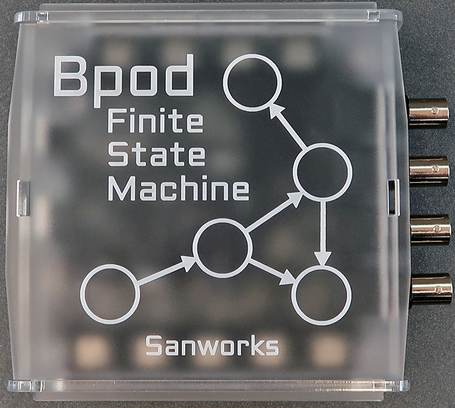
\includegraphics[height=1em]{icons/bpod.jpg}} PyBpod}, a programming interface for the Bpod: a system for precise measurement of small animal behavior.
      \begin{itemize}
        \setlength\itemsep{-0.3em}
        \item Implemented emulator functionality for the Bpod device. See my contributions to the \href{https://github.com/ckaraneen/pybpod}{pybpod submodules}.
        \item Created v1 of the 2AFC experimental neuroscience protocol. See \href{https://github.com/ckaraneen/mouse2afc}{mouse2afc}.
      \end{itemize}
    \resumeSubHeadingListEnd

%-----------SUPERVISOR EXPERIENCE-----------------
\section{Supervisor Experience}
  \begin{itemize}
    \item \textit{\href{https://www.linkedin.com/in/henry-flynn/}{Henry J. Flynn}} @ \hyperref[PoiraziLabMarker]{Poirazi Lab}, \textit{April -- Aug. 2023}: \href{https://drexel.edu/}{{\raisebox{-0.2em}{
\includegraphics[height=1em]{icons/drexel.jpg}}} Drexel University} student who under my supervision built upon my \hyperref[PoiraziLabVolMarker]{volunteer contribution} and improved the \href{https://github.com/Poirazi-Lab/mouse2afc}{Mouse2AFC protocol}.
  \end{itemize}

%-----------AWARDS, FELLOWSHIPS & FUNDING-----------------
\section{Awards, Fellowships \& Funding}
\begin{itemize}
  \item 2023 -- 2024
    \setlength\itemsep{-0.3em}
    \begin{itemize}
      \item \textit{\hyperref[BrainNeuroAIWorkshop2024PosterMarker]{BRAIN NeuroAI Early-Career Scholar}}, NIH/DARPA \textbf{honorarium} (\textit{Nov. 12 -- 13, 2024}): \$400
      \item \textit{\href{https://www.cshl.edu/research/neuroscience/neuroai/}{CSHL NeuroAI Program}} \textbf{funding} (\textit{June -- Nov. 2024}, \hyperref[BanerjeeLabMarker]{Banerjee Lab})\label{CSHLNeuroAIResearchInternFundingMarker}: \$40000
      \item \textit{\href{https://erasmus-plus.ec.europa.eu/opportunities/opportunities-for-individuals/students/traineeships-abroad-for-students}{Erasmus+}}/\href{https://www.iky.gr/en/discover-erasmus}{IKY} \textbf{funding} (\textit{June -- Aug. 2024}, \hyperref[BanerjeeLabMarker]{CSHL travel \& stay}): 3600\euro
      \item \textit{IMBB-FoRTH} MSc \textbf{fellowships} (\textit{July 2023 -- April 2024}, \hyperref[PoiraziLabMarker]{Poirazi Lab})\label{IMBBFoRTHFellowshipMarker}: 5000\euro
    \end{itemize}
  \item 2022 -- 2023
    \setlength\itemsep{-0.3em}
    \begin{itemize}
        \item \textit{\href{https://global.upenn.edu/isss/j1scholar}{UPenn Visiting Scholar}} \textbf{funding} (\textit{Dec. 2022 -- March 2023}, \hyperref[KordingLabMarker]{Kording Lab}) \label{UPennVisitingScholarFundingMarker}: \$6000
        \item \textit{\href{https://erasmus-plus.ec.europa.eu/opportunities/opportunities-for-individuals/students/traineeships-abroad-for-students}{Erasmus+}}/\href{https://www.iky.gr/en/discover-erasmus}{IKY} \textbf{funding} (\textit{Dec. 2022 -- March 2023}, \hyperref[KordingLabMarker]{UPenn travel \& stay}): 4500\euro
    \end{itemize}
\end{itemize}

%-----------CONFERENCES, WORKSHOPS & SUMMER SCHOOLS-----------------
\section{Conferences, Workshops \& Summer Schools}
  \begin{itemize}
    \item \label{BrainNeuroAIWorkshop2024PosterMarker} \href{https://n4solutionsllc.com/brainneuroai/}{{
    \raisebox{-0.55em}{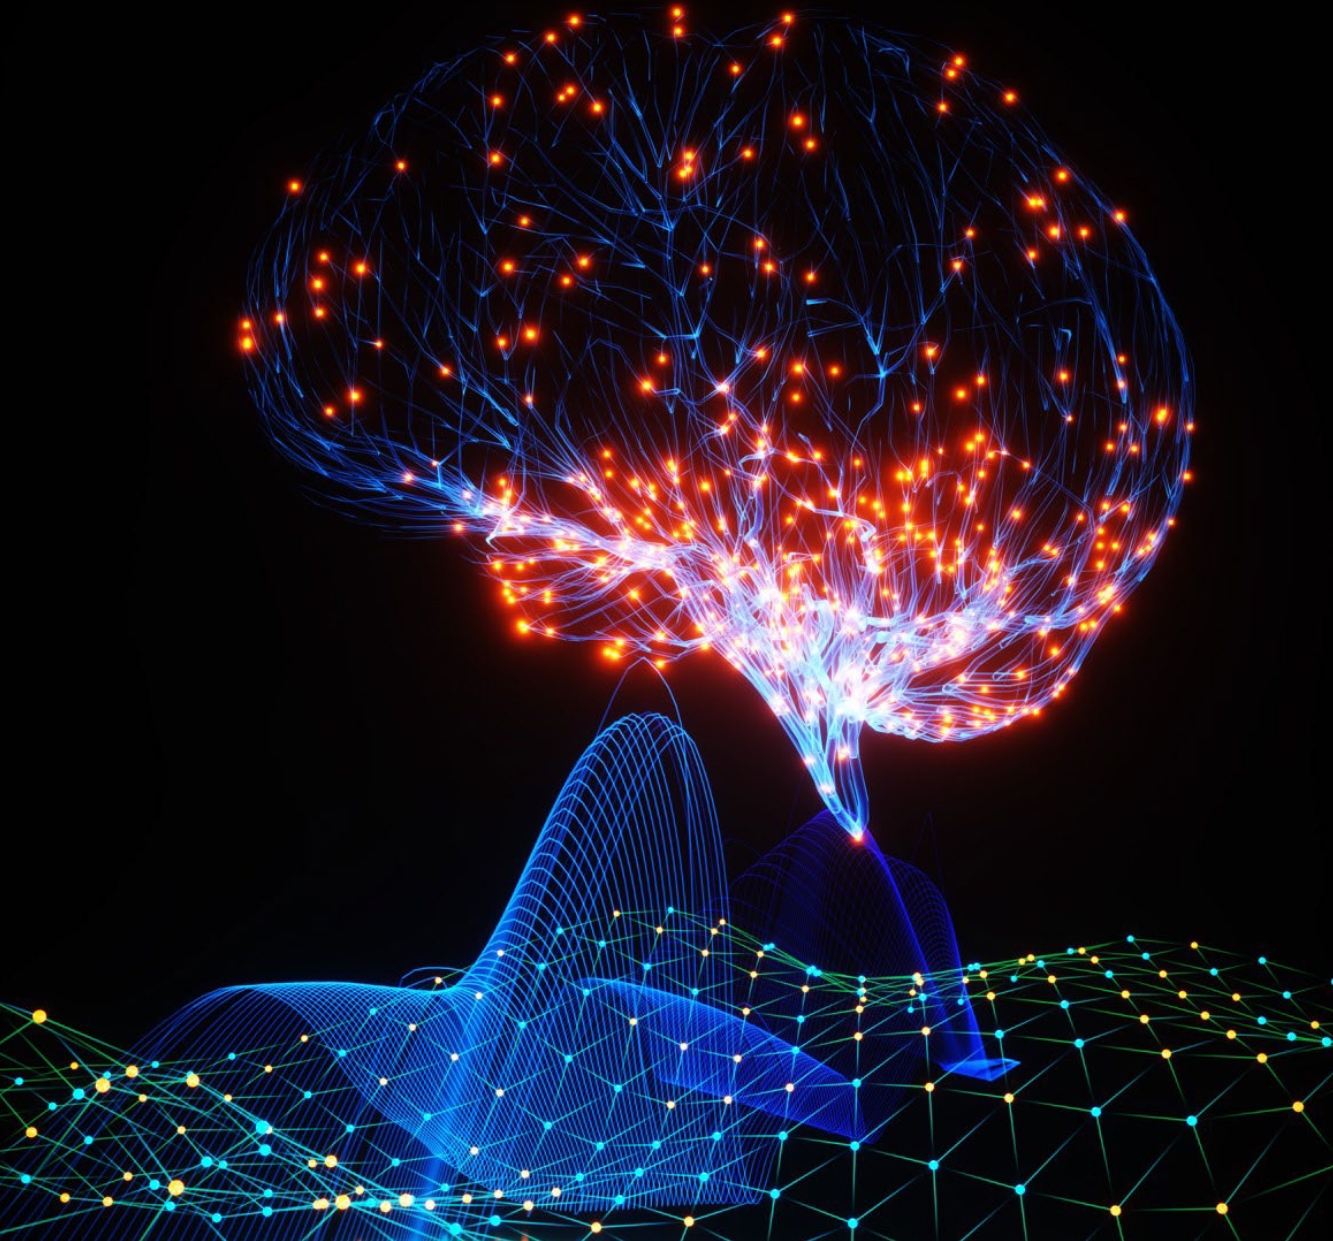
\includegraphics[height=2.5em]{icons/brain_neuroai_workshop.png}}} \textit{BRAIN NeuroAI Workshop 2024}} \textbf{@} \href{https://www.nih.gov/}{\raisebox{-0.6em}{
\includegraphics[height=2.2em]{icons/nih.png}}}, Bethesda, Maryland, USA (\href{https://raw.githubusercontent.com/ckaraneen/brain-neuroai-workshop-2024/main/poster.pdf}{\textbf{poster}})
    \item \href{https://meetings.cshl.edu/meetings.aspx?meet=NAISYS&year=24}{{{\raisebox{-0.6em}{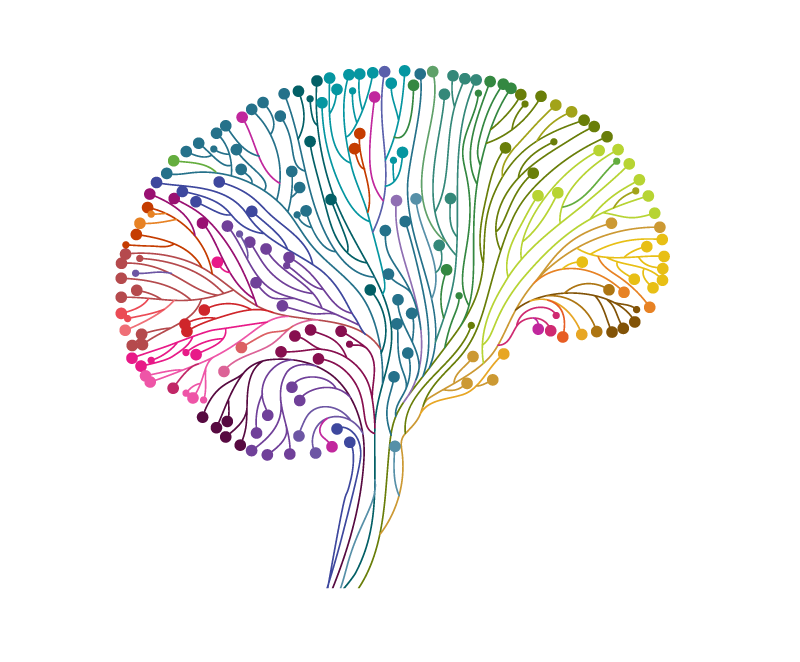
\includegraphics[height=2.2em]{icons/naisys.png}}}}NAISys2024}: \textit{From Neuroscience to Artificial Intelligence 2024} \textbf{@} \href{https://www.cshl.edu/}{\raisebox{-0.3em}{
\includegraphics[height=1.5em]{icons/cshl.png}}}, New York, USA
    \item \label{MLSS2024PosterMarker} \href{https://groups.oist.jp/mlss}{{{\raisebox{-0.04em}{
\includegraphics[height=0.75em]{icons/mlss.jpg}}}}2024}: \textit{Machine Learning Summer School 2024} \textbf{@} \href{https://www.oist.jp/}{\raisebox{-0.6em}{
\includegraphics[height=2.2em]{icons/oist.png}}}, Okinawa, Japan (\href{https://raw.githubusercontent.com/ckaraneen/mlss2024/main/poster.pdf}{\textbf{poster}})
  \end{itemize}

%-----------PUBLICATIONS-----------------
\section{Publications}
\begin{enumerate}
\item \label{NeuroscienceMScThesisMarker} Christos Karageorgiou Kaneen, ``\textit{Meta-learning synaptic plasticity rules to approximate gradient descent}'', M.Sc. Thesis, School of Medicine, University of Crete, Heraklion, Greece, 2024 (\url{https://elocus.lib.uoc.gr/dlib/0/c/8/metadata-dlib-1713262345-844945-28206.tkl})
\item Christos Karageorgiou Kaneen, ``\textit{Methodology for designing GDPR compliant IoT applications}'', M.Eng. Thesis, School of Electrical and Computer Engineering, Technical University of Crete, Chania, Greece, 2019 (\url{https://doi.org/10.26233/heallink.tuc.84151})
\item Christos Karageorgiou Kaneen, E.G.M. Petrakis, ``\textit{Towards evaluating GDPR compliance in IoT applications}'', Procedia Computer Science, Volume 176, 2020, Pages 2989-2998 (\url{https://doi.org/10.1016/j.procs.2020.09.204})
\end{enumerate}

\blfootnote{\large{Last update: \textit{\today}. For latest CV, \href{https://raw.githubusercontent.com/ckaraneen/cv/master/cv.pdf}{\textbf{click here}}.}}
\end{document}
